% !TEX program = lualatex
% !BIB program = bibtex
\RequirePackage{luatex85}
\PassOptionsToPackage{unicode}{hyperref}
\PassOptionsToPackage{naturalnames}{hyperref}
\documentclass{article}
% \usepackage{geometry}
\usepackage{fullpage}
\usepackage{parskip}
\usepackage{physics}
\usepackage{amsmath}
\usepackage{amssymb}
\usepackage{xcolor}
\usepackage[colorlinks,linkcolor=blue,citecolor=green]{hyperref}
\usepackage{array}
\usepackage{longtable}
\usepackage{multirow}
\usepackage{comment}
\usepackage{graphicx}
\usepackage{cite}
\usepackage{amsfonts}
\usepackage{bm}
\usepackage{slashed}
\usepackage{dsfont}
\usepackage{mathtools}
\usepackage[compat=1.1.0]{tikz-feynman}
\usepackage{simplewick}
\usepackage{mathrsfs}
\usepackage{xparse}
\usepackage{enumerate}
\usepackage{extarrows}

\allowdisplaybreaks

\newcommand{\calA}{\mathcal{A}}
\newcommand{\mm}[1]{\frac{\dd^4#1}{(2\pi)^4}}
\newcommand{\mme}[1]{\frac{\dd^3\vb{#1}}{(2\pi)^3}}
\newcommand{\mmd}[2][d]{\frac{\dd^{#1}{#2}}{(2\pi)^{#1}}}
\newcommand{\red}[1]{{\color{red}#1}}

\usepackage{shellesc}
\usetikzlibrary{external}
% \usepgfplotslibrary{external}
\tikzexternalize[shell escape=-enable-write18,prefix=./,system call={lualatex \tikzexternalcheckshellescape -halt-on-error -interaction=batchmode -jobname "\image" "\texsource"},up to date check=diff]

\title{Note on Braaten's Paper}
\author{Yingsheng Huang}
\begin{document}
    \maketitle
    
    \section{Intro}
    Hamiltonian\cite{Braaten2008}: 
    \begin{align}
        \mathcal{H}=\sum_\sigma\frac{1}{2m}\nabla\psi_\sigma^{\dagger}\cdot\nabla\psi_\sigma^{(\Lambda)}+\frac{g(\Lambda)}{m}\psi^\dagger_1\psi^\dagger_2\psi_3\psi_4^{(\Lambda)}+\mathcal{V}
    \end{align}
    where the renormalized coupling 
    \begin{align}
        g(\Lambda)=\frac{4\pi a}{1-2a\Lambda/\pi}
        \label{gL}
    \end{align}

    \section{Amplitude}
    Consider: 
    \begin{align}
        i\calA=\mel{34}{\psi^\dagger\psi}{12}=
        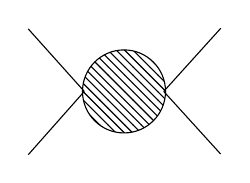
\begin{tikzpicture}[baseline=(o1.base)]
            \begin{feynman}
                \diagram[small,horizontal=o1 to o3]{
                    p1 -- o1 --[draw=none] o3 -- p3;
                    p2 -- o1 --[draw=none] o3 -- p4;
                };
                \node[blob, minimum size=30pt] at ($(o1)!0.5!(o3)$) (o2);
            \end{feynman}
        \end{tikzpicture}
    \end{align}
    Define $P=p_1+p_2=(E,\vb{0})$, and $E=p^2/m$. 
    The integral equation is 
    \begin{align}
        i\calA=-\frac{ig(\Lambda)}{m}\pqty{1+i\calA\int\mm{k}\frac{i}{k^0-\frac{\vb{k}^2}{2m}+i\epsilon}\frac{i}{P^0-k^0-\frac{\abs{\vb{k-P}}^2}{2m}+i\epsilon}}
    \end{align}
    The integral gives (redefine $\epsilon\rightarrow2m\epsilon$)
    \begin{align}
        \mathcal{I}=\frac{i m }{2 \pi ^2}\left(-\Lambda +\sqrt{ -mE-i \epsilon } \tan ^{-1}\left(\frac{\Lambda }{\sqrt{ -mE-i \epsilon }}\right)\right)=-\frac{i \Lambda  m}{2 \pi ^2}+\frac{m p}{4 \pi }
    \end{align}
    and 
    \begin{align}
        i\calA&=\frac{-1}{\mathcal{I}+\frac{m}{ig(\Lambda)}}=-\bqty{\frac{i m \sqrt{-mE -i \epsilon } \tan ^{-1}\left(\frac{\Lambda }{\sqrt{-mE -i \epsilon }}\right)}{2 \pi ^2}-\frac{i m}{4 \pi  a}}^{-1}\\
        &\xlongequal{\Lambda\rightarrow\infty}\frac{4 i \pi/m  }{-1/a+ \sqrt{-mE -i \epsilon }}
    \end{align}

    Note that by definition, scattering length is the leading order momentum expansion of $1/\calA$, which gives 
    \begin{align}
        \frac{1}{a}&=\frac{4i\pi}{m}\pqty{\mathcal{I}+\frac{m}{ig(\Lambda)}}^{(0)}\\
        &=\frac{4 \pi }{g(\Lambda)}+\frac{2 \Lambda }{\pi }\\
        &\hspace{-0.4in}\Rightarrow g(\Lambda)=\frac{4 \pi  a}{1 -2 a \Lambda/\pi }
    \end{align}
    and this is actually how we get the form of \eqref{gL}. 

    \section{OPE}
    \subsection{l.h.s.}
    Take what we got in the last section as a new non-perturbative vertex, we only need to deal with tree diagram this way. First we have Figure~2(a) in Braaten's paper: 
    \begin{align}
        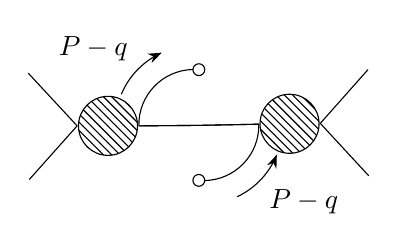
\begin{tikzpicture}[baseline=(o1.base)]
            \begin{feynman}
                \diagram[small,horizontal=o1 to o3]{
                    p1 -- o1 --[draw=none] o3 -- o35 -- o4 --[draw=none] o6 -- p3;
                    p2 -- o1 --[draw=none] o3 -- o35 -- o4 --[draw=none] o6 -- p4;
                };
                \node[empty dot] at ($(o3)!0.5!(o4)+(0,20pt)$) (ps1);
                \node[empty dot] at ($(o3)!0.5!(o4)+(0,-20pt)$) (ps2);
                \diagram*{
                    (o3) --[quarter left,momentum={[arrow shorten=0.25]\(P-q\)}] (ps1);
                    (ps2) --[quarter right,momentum'={[arrow shorten=0.25]\(P-q\)}] (o4);
                };
                \node[blob] at ($(o1)!0.5!(o3)$) (o2);
                \node[blob] at ($(o4)!0.5!(o6)$) (o5);
            \end{feynman}
        \end{tikzpicture}&=\mel{34}{\psi^\dagger\left(-\frac{\vb{r}}{2}\right)\psi\left(\frac{\vb{r}}{2}\right)}{12}\\
        &=(i\calA)^2\int\frac{\dd^4q}{(2\pi)^4}\frac{i}{q^0-\frac{\vb{q}^2}{2m}+i\epsilon}\frac{i}{\bqty{E-q^0-\frac{\vb{q}^2}{2m}+i\epsilon}^2}e^{i\vb{q}\cdot\vb{r}}\\
        &=\calA^2\int\frac{\dd^3\vb{q}}{(2\pi)^3}\frac{m^2e^{i\vb{q}\cdot\vb{r}}}{\pqty{\vb{q}^2-p^2-i\epsilon}^2}\\
        &=\frac{i m^2\calA^2 e^{i p r}}{8 \pi  p}
    \end{align}
    \subsection{r.h.s.}
    For simplicity, we drop the external lines and focus on the internal subgraph. Consider Figure~2(b):
    \begin{align}
        &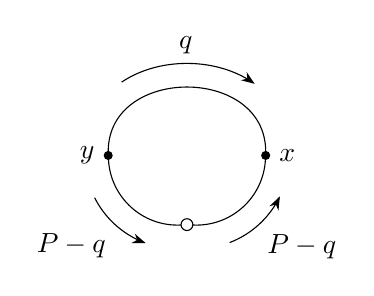
\begin{tikzpicture}[baseline=(o3.base)]
            \begin{feynman}
                \diagram[small,horizontal=o3 to o4,layered layout]{
                    o3[dot,label=180:\(y\)] --[draw=none] o35 --[draw=none] o4[dot,label=0:\(x\)];
                };
                \vertex at ($(o3)!0.5!(o4)+(0,25pt)$) (ps1);
                \node[empty dot] at ($(o3)!0.5!(o4)+(0,-25pt)$) (ps2);
                \diagram*{
                    (o3) --[half left,looseness=1.4,momentum={[arrow shorten=0.25]\(q\)}] (o4);
                    (o3) --[quarter right,momentum'={[arrow shorten=0.25]\(P-q\)}] (ps2);
                    (ps2) --[quarter right,momentum'={[arrow shorten=0.25]\(P-q\)}] (o4);
                };
            \end{feynman}
        \end{tikzpicture}=\mel{34}{\psi^\dagger\psi\left(0\right)}{12}_{amp}\\
        &=\int\dd^4x\int\dd^4y\int\mm{l_1}\mm{l_2}\mm{q}e^{iP\cdot y}e^{-iP\cdot x}e^{-il_1\cdot y}e^{il_2\cdot x}e^{iq\cdot (x-y)}\tilde D(l_1)\tilde D(l_2)\tilde D(q)\\
        &=\int\mm{q}\tilde D(P-q)\tilde D(P-q)\tilde D(q)\\
        &=-\int\mme{q}\frac{m^2}{\pqty{\vb{q}^2-p^2-i\epsilon}^2}\\
        &=-\frac{im^2}{8\pi p}
    \end{align}
    where $\tilde D$ marks momentum space propagator and two external vertexes give an $(i\calA)^2$ factor. The total contribution is 
    \begin{align}
        \frac{im^2\calA^2}{8\pi p},
    \end{align}
    the first order Fourier expansion of the l.h.s. 
    \subsection{Higher dimensional operators}
    Figure~2(c) gives
    \begin{align}
        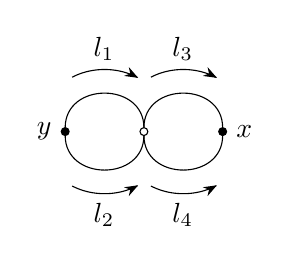
\begin{tikzpicture}[baseline=(o3.base)]
            \begin{feynman}
                \diagram[small,horizontal=o3 to o4,layered layout]{
                    o3[dot,label=180:\(y\)] --[half left,momentum={[arrow shorten=0.3]\(l_1\)}] o35[empty dot] --[half left,momentum={[arrow shorten=0.3]\(l_3\)}] o4[dot,label=0:\(x\)];
                    o3 --[half right,momentum'={[arrow shorten=0.3]\(l_2\)}] o35 --[half right,momentum'={[arrow shorten=0.3]\(l_4\)}] o4;
                };
            \end{feynman}
        \end{tikzpicture}&=\mel{34}{\psi^\dagger\psi^\dagger\psi\psi\left(0\right)}{12}_{amp}\\
        &=\int\dd^4x\int\dd^4y\int\mm{l_1}\mm{l_2}\mm{l_3}\mm{l_4}e^{iP\cdot y}e^{-iP\cdot x}e^{-i(l_1+l_2)\cdot y}e^{i(l_3+l_4)\cdot x}\notag\\
        &\tilde D(l_1)\tilde D(l_2)\tilde D(l_3)\tilde D(l_4)
    \end{align}
    which becomes
    \begin{align}
        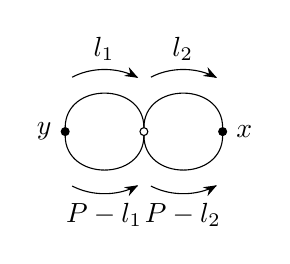
\begin{tikzpicture}[baseline=(o3.base)]
            \begin{feynman}
                \diagram[small,horizontal=o3 to o4,layered layout]{
                    o3[dot,label=180:\(y\)] --[half left,momentum={[arrow shorten=0.3]\(l_1\)}] o35[empty dot] --[half left,momentum={[arrow shorten=0.3]\(l_2\)}] o4[dot,label=0:\(x\)];
                    o3 --[half right,momentum'={[arrow shorten=0.3]\(P-l_1\)}] o35 --[half right,momentum'={[arrow shorten=0.3]\(P-l_2\)}] o4;
                };
            \end{feynman}
        \end{tikzpicture}&=\int\mm{l_1}\mm{l_2}\tilde D(l_1)\tilde D(P-l_1)\tilde D(l_2)\tilde D(P-l_2)\\
        &=-\int\mme{l_1}\mme{l_2}\frac{m^2}{\left(\vb{l_1}^2-p^2-i \epsilon \right) \left(\vb{l_2}^2-p^2-i \epsilon \right)}\\
        &=-\mathcal{I}^2
    \end{align}
    There're four diagrams in total: 
    \begin{align}
        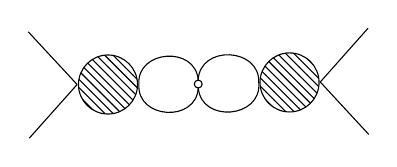
\begin{tikzpicture}[baseline=(o1.base)]
            \begin{feynman}
                \diagram[small,horizontal=o1 to o3]{
                    p1 -- o1 --[draw=none] o3 --[draw=none] o35[empty dot] --[draw=none] o4 --[draw=none] o6 -- p3;
                    p2 -- o1 --[draw=none] o3 --[draw=none] o35 --[draw=none] o4 --[draw=none] o6 -- p4;
                };
                \diagram*{
                    (o3) --[half left] (o35) --[half left] (o4);
                    (o3) --[half right] (o35) --[half right] (o4);
                };
                \node[blob] at ($(o1)!0.5!(o3)$) (o2);
                \node[blob] at ($(o4)!0.5!(o6)$) (o5);
            \end{feynman}
        \end{tikzpicture}&=\calA^2\mathcal{I}^2\\
        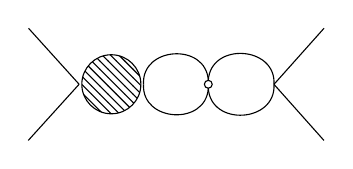
\begin{tikzpicture}[baseline=(o1.base)]
            \begin{feynman}
                \diagram[small,horizontal=o1 to o3]{
                    p1 -- o1 --[draw=none] o3 --[draw=none] o35[empty dot] --[draw=none] o4 -- p3;
                    p2 -- o1 --[draw=none] o3 --[draw=none] o35 --[draw=none] o4 -- p4;
                };
                \diagram*{
                    (o3) --[half left] (o35) --[half left] (o4);
                    (o3) --[half right] (o35) --[half right] (o4);
                };
                \node[blob] at ($(o1)!0.5!(o3)$) (o2);
            \end{feynman}
        \end{tikzpicture}&=\calA\mathcal{I}\\
        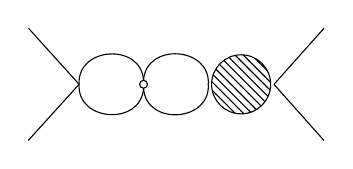
\begin{tikzpicture}[baseline=(o3.base)]
            \begin{feynman}
                \diagram[small,horizontal=o3 to o4]{
                    p1 -- o3 --[draw=none] o35[empty dot] --[draw=none] o4 --[draw=none] o6 -- p3;
                    p2 -- o3 --[draw=none] o35 --[draw=none] o4 --[draw=none] o6 -- p4;
                };
                \diagram*{
                    (o3) --[half left] (o35) --[half left] (o4);
                    (o3) --[half right] (o35) --[half right] (o4);
                };
                \node[blob] at ($(o4)!0.5!(o6)$) (o5);
            \end{feynman}
        \end{tikzpicture}&=\calA\mathcal{I}\\
        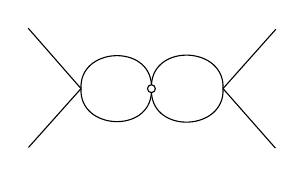
\begin{tikzpicture}[baseline=(o3.base)]
            \begin{feynman}
                \diagram[small,horizontal=o3 to o4]{
                    p1 -- o3 --[draw=none] o35[empty dot] --[draw=none] o4 -- p3;
                    p2 -- o3 --[draw=none] o35 --[draw=none] o4 -- p4;
                };
                \diagram*{
                    (o3) --[half left] (o35) --[half left] (o4);
                    (o3) --[half right] (o35) --[half right] (o4);
                };
            \end{feynman}
        \end{tikzpicture}&=1
    \end{align}
    We have 
    \begin{align}
        \expval{\psi^\dagger_1\psi^\dagger_2\psi_1\psi_2^{(\Lambda)}(0)}_{\pm\vb{p}}=(\calA\mathcal{I}+1)^2
    \end{align}
    in total. Plug in 
    \begin{align}
        \mathcal{I}=-\frac{m}{ig(\Lambda)}-\frac{1}{\calA}
    \end{align}
    we have
    \begin{align}
        \expval{\psi^\dagger_1\psi^\dagger_2\psi_1\psi_2^{(\Lambda)}(0)}_{\pm\vb{p}}=m^2g^{-2}(\Lambda)\calA^2
        \label{2c}
    \end{align}
    The Wilson coefficient must be 
    \begin{align}
        -\frac{r}{8\pi}g^2(\Lambda)
    \end{align}

    \section{Contact}
    \subsection{Definition}
    \begin{align}
        C=\int\dd^3R\expval{g^2\psi^\dagger_1\psi^\dagger_2\psi_1\psi_2(R)}
        \label{contact}
    \end{align}
    \subsection{Energy Relation}
    According to the Hamiltonian: 
    \begin{align}
    \mathcal{H} = \left(\sum_{\sigma} \frac {1} {2 m} \nabla \psi_{\sigma}^{\dagger} \cdot \nabla \psi_{\sigma}^{(\Lambda)} - \frac {\Lambda} {2 \pi^{2} m} g^{2}(\Lambda) \psi_{1}^{\dagger} \psi_{2}^{\dagger} \psi_{1} \psi_{2}\right){+ \frac {1} {4 \pi m a} g^{2}(\Lambda) \psi_{1}^{\dagger} \psi_{2}^{\dagger} \psi_{1} \psi_{2} + \mathcal{V}}
    \end{align}
    where the matrix elements of those three operators are finite. The $\nabla \psi_{\sigma}^{\dagger} \cdot \nabla \psi_{\sigma}^{(\Lambda)}$ part gives a linear divergence $2\times\frac{\Lambda  m\calA^2}{4 \pi ^2}$ for two spin states in total while the other one gives $-\frac{\Lambda m\calA^2}{2\pi^2}$, we can see that the linear divergence is cancelled. Integrating over positions, we obtain
    \begin{align}
        &\int\dd^3R\expval{\nabla \psi_{\sigma}^{\dagger} \cdot \nabla \psi_{\sigma}}=\int\dd^3R\dd^3r\delta^{(3)}(\vb{r})\expval{\nabla \psi_{\sigma}^{\dagger}(\vb{R-\frac{r}{2}}) \cdot \nabla \psi_{\sigma}(\vb{R+\frac{r}{2}})} =\int\mme{k}k^2\rho_\sigma(k)\\
        &\frac {1} {4 \pi m a} \int\dd^3R \expval{g^{2}\psi_{1}^{\dagger} \psi_{2}^{\dagger} \psi_{1} \psi_{2}}=\frac {1} {4 \pi m a}C
    \end{align}
    also notice
    \begin{align}
        \int^\Lambda\mme{k}\frac{1}{\vb{k}^2}=\frac{\Lambda}{2\pi^2}
    \end{align}
    we have
    \begin{align}
        \int\dd^3R\frac {\Lambda} {2 \pi^{2} m} \expval{g^{2} \psi_{1}^{\dagger} \psi_{2}^{\dagger} \psi_{1} \psi_{2}}=\sum_\sigma\int\mme{k}\frac{k^2}{2m}\frac{C}{\vb{k}^4}
    \end{align}
    we achieve 
    \begin{align}
        E = \sum_{\sigma} \int \frac {d^{3} k} {(2 \pi)^{3}} \frac {k^{2}} {2 m} \left(\rho_{\sigma} (k) - \frac {C} {k^{4}}\right) + \frac {C} {4 \pi m a}+ \int d^{3} R \langle V \rangle
    \end{align}
    \subsection{Adiabatic relation}
    Using F-H theorem
    \begin{align}
        \dd E / \dd a = \int \dd^{3} R \langle \partial \mathcal{H} / \partial a \rangle
    \end{align}
    it's straightforward that
    \begin{align}
        \partial \mathcal{H} / \partial a = g^{2} \psi_{1}^{\dagger} \psi_{2}^{\dagger} \psi_{1} \psi_{2} / (4 \pi m a^{2})
    \end{align}
    We then have 
    \begin{align}
        \frac {\dd E} {\dd (1 / a)} = - \frac {1} {4 \pi m} C
    \end{align}
    using \eqref{contact}. 
    \subsection{Viral Theorem}
    Dimensional analysis requires 
    \begin{align}
        \bqty{\omega\pdv{\omega}-\frac{1}{2}a\pdv{a}}\int\dd^3R\expval{\mathcal{H}}=1
    \end{align}
    Together with F-H theorem 
    \begin{align}
        &\frac{a}{2}\pdv{a}\int\dd^3R\expval{\mathcal{H}}=\frac{C}{8\pi m a}+\frac{a}{2}\pdv{a}\expval{\mathcal{V}}==\frac{a}{2}\dv{E}{a}\\
        &\pdv{\omega}\int\dd^3R\expval{\mathcal{H}}=\pdv{\omega}\expval{\mathcal{V}}=\dv{E}{\omega}
    \end{align}

    \subsection{OPE for number density operators}
    We have a pair of number density operators
    \begin{align}
        \psi_1^\dagger\psi_1(\vb{R}-\frac{1}{2}\vb{r})\;\&\; \psi_2^\dagger\psi_2(\vb{R}+\frac{1}{2}\vb{r})
    \end{align}
    and the diagram is 
    \begin{align}
        &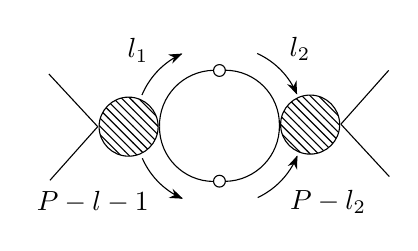
\begin{tikzpicture}[baseline=(o1.base)]
            \begin{feynman}
                \diagram[small,horizontal=o1 to o3]{
                    p1 -- o1 --[draw=none] o3 --[draw=none] o35 --[draw=none] o4 --[draw=none] o6 -- p3;
                    p2 -- o1 --[draw=none] o3 --[draw=none] o35 --[draw=none] o4 --[draw=none] o6 -- p4;
                };
                \node[empty dot] at ($(o3)!0.5!(o4)+(0,20pt)$) (ps1);
                \node[empty dot] at ($(o3)!0.5!(o4)+(0,-20pt)$) (ps2);
                \diagram*{
                    (o3) --[quarter left,momentum={[arrow shorten=0.25]\(l_1\)}] (ps1);
                    (ps1) --[quarter left,momentum={[arrow shorten=0.25]\(l_2\)}] (o4);
                    (o3) --[quarter right,momentum'={[arrow shorten=0.25]\(P-l-1\)}] (ps2);
                    (ps2) --[quarter right,momentum'={[arrow shorten=0.25]\(P-l_2\)}] (o4);
                };
                \node[blob] at ($(o1)!0.5!(o3)$) (o2);
                \node[blob] at ($(o4)!0.5!(o6)$) (o5);
            \end{feynman}
        \end{tikzpicture}\\
        &=(i\calA)^2\int\mm{l_1}\mm{l_2}\frac{i}{l_1^0-\frac{\vb{l_1}^2}{2m}+i\epsilon}\frac{i}{{E-l_1^0-\frac{\vb{l_1}^2}{2m}+i\epsilon}}\frac{i}{l_2^0-\frac{\vb{l_2}^2}{2m}+i\epsilon}\frac{i}{{E-l_2^0-\frac{\vb{l_2}^2}{2m}+i\epsilon}}e^{i\vb{q}\cdot\vb{r}}\\
        &=\frac{\calA^2m^2 }{16 \pi ^2 r^2}e^{2 i p r}
    \end{align}
    Compare with the result of Figure~2(c) \eqref{2c} we have the Wilson coefficient
    \begin{align}
        \frac{g^2(\Lambda)}{16 \pi ^2 r^2}
    \end{align}

    \section{Reformulate in Dimensional Regularization}
    The renormalized Hamiltonian reads
    \begin{align}
        \mathcal{H}=\sum_\sigma\frac{1}{2m}\nabla\psi_\sigma^{\dagger}\cdot\nabla\psi_\sigma+Z_g\frac{g}{m}\psi^\dagger_1\psi^\dagger_2\psi_3\psi_4
    \end{align}
    We have 
    \begin{align}
        i\calA=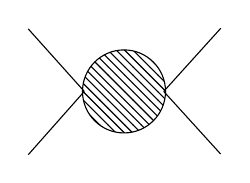
\begin{tikzpicture}[baseline=(o1.base)]
            \begin{feynman}
                \diagram[small,horizontal=o1 to o3]{
                    p1 -- o1 --[draw=none] o3 -- p3;
                    p2 -- o1 --[draw=none] o3 -- p4;
                };
                \node[blob, minimum size=30pt] at ($(o1)!0.5!(o3)$) (o2);
            \end{feynman}
        \end{tikzpicture}
        % +
        % \begin{tikzpicture}[baseline=(o1.base)]
        %     \begin{feynman}
        %         \diagram[small,layered layout]{
        %             p1 -- o1 -- p3;
        %             p2 -- o1 -- p4;
        %         };
        %         \node[crossed dot] at (o1);
        %     \end{feynman}
        % \end{tikzpicture}+\cdots
        \\
        \mathcal{I}\equiv
        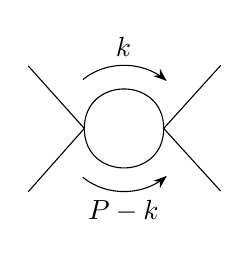
\begin{tikzpicture}[baseline=(o1.base)]
            \begin{feynman}
                \diagram[small,horizontal=o1 to o4]{
                    p1 -- o1 --[draw=none] o4 -- p3;
                    p2 -- o1 --[draw=none] o4 -- p4;
                };
                \diagram*{
                    (o1) --[half left,looseness=1.7,momentum={[arrow shorten=0.25]\(k\)}] (o4);
                    (o1) --[half right,looseness=1.7,momentum'={[arrow shorten=0.25]\(P-k\)}] (o4);
                };
            \end{feynman}
        \end{tikzpicture}
    \end{align}
    The integral equation is 
    \begin{align}
        i\calA=-\frac{iZ_gg}{m}\pqty{1+i\calA\mathcal{I}}
    \end{align}
    \begin{align}
        \mathcal{I}\equiv\int\mmd[d+1]{k}\frac{i}{k^0-\frac{\vb{k}^2}{2m}+i\epsilon}\frac{i}{P^0-k^0-\frac{\abs{\vb{k-P}}^2}{2m}+i\epsilon}
    \end{align}
    Graphically we have
    \begin{align*}
        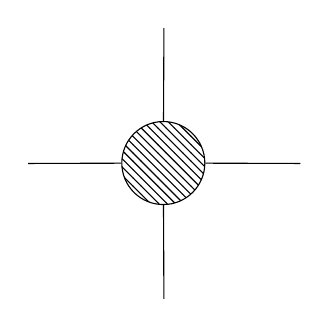
\begin{tikzpicture}[baseline=(o1.base)]
            \begin{feynman}
                \diagram[small,horizontal=p1 to p3]{
                    p1 -- o1[blob, minimum size=30pt] -- p3;
                    p2 -- o1 -- p4;
                };
                % \node[blob, minimum size=30pt] at (o1);
            \end{feynman}
        \end{tikzpicture}=
        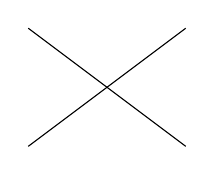
\begin{tikzpicture}[baseline=(o3.base)]
            \begin{feynman}
                \diagram[small,layered layout,horizontal=p1 to p3]{
                    p1 -- o3 -- p3;
                    p2 -- o3 -- p4;
                };
                \node at (o3);
            \end{feynman}
        \end{tikzpicture}+
        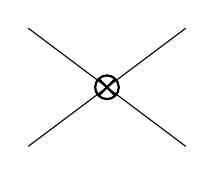
\begin{tikzpicture}[baseline=(o3.base)]
            \begin{feynman}
                \diagram[small,layered layout,horizontal=p1 to p3]{
                    p1 -- o3 -- p3;
                    p2 -- o3 -- p4;
                };
                \node[crossed dot,style=thick] at (o3);
            \end{feynman}
        \end{tikzpicture}+
        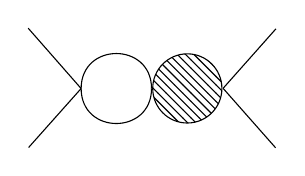
\begin{tikzpicture}[baseline=(o3.base)]
            \begin{feynman}
                \diagram[small,horizontal=o3 to o4]{
                    p1 -- o3 --[draw=none] o4 --[draw=none] o6 -- p3;
                    p2 -- o3 --[draw=none] o4 --[draw=none] o6 -- p4;
                };
                \diagram*{
                    (o3) --[half left,looseness=1.7] (o4);
                    (o3) --[half right,looseness=1.7] (o4);
                };
                \node[blob, minimum size=25pt] at ($(o4)!0.5!(o6)$) (o5);
            \end{feynman}
        \end{tikzpicture}+
        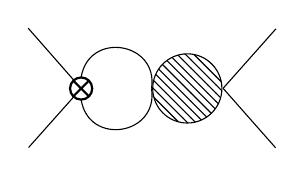
\begin{tikzpicture}[baseline=(o3.base)]
            \begin{feynman}
                \diagram[small,horizontal=o3 to o4]{
                    p1 -- o3[crossed dot, minimum size=8pt,style=thick] --[draw=none] o4 --[draw=none] o6 -- p3;
                    p2 -- o3 --[draw=none] o4 --[draw=none] o6 -- p4;
                };
                \diagram*{
                    (o3) --[half left,looseness=1.7] (o4);
                    (o3) --[half right,looseness=1.7] (o4);
                };
                \node[blob, minimum size=25pt] at ($(o4)!0.5!(o6)$) (o5);
            \end{feynman}
        \end{tikzpicture}
    \end{align*}
    or 
    \begin{align*}
        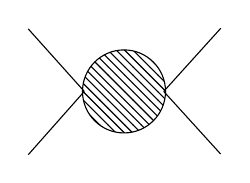
\begin{tikzpicture}[baseline=(o1.base)]
            \begin{feynman}
                \diagram[small,horizontal=o1 to o3]{
                    p1 -- o1 --[draw=none] o3 -- p3;
                    p2 -- o1 --[draw=none] o3 -- p4;
                };
                \node[blob, minimum size=30pt] at ($(o1)!0.5!(o3)$) (o2);
            \end{feynman}
        \end{tikzpicture}&=
        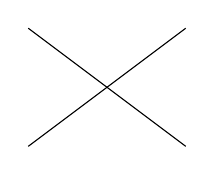
\begin{tikzpicture}[baseline=(o3.base)]
            \begin{feynman}
                \diagram[small,layered layout,horizontal=p1 to p3]{
                    p1 -- o3 -- p3;
                    p2 -- o3 -- p4;
                };
                \node at (o3);
            \end{feynman}
        \end{tikzpicture}+
        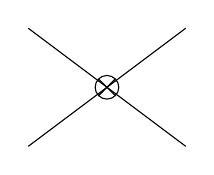
\begin{tikzpicture}[baseline=(o3.base)]
            \begin{feynman}
                \diagram[small,layered layout,horizontal=p1 to p3]{
                    p1 -- o3 -- p3;
                    p2 -- o3 -- p4;
                };
                \node[crossed dot] at (o3);
            \end{feynman}
        \end{tikzpicture}+
        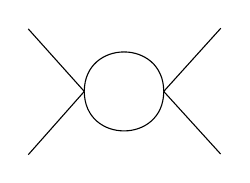
\begin{tikzpicture}[baseline=(o1.base)]
            \begin{feynman}
                \diagram[small,horizontal=o1 to o4]{
                    p1 -- o1 --[draw=none] o4 -- p3;
                    p2 -- o1 --[draw=none] o4 -- p4;
                };
                \diagram*{
                    (o1) --[half left,looseness=1.7] (o4);
                    (o1) --[half right,looseness=1.7] (o4);
                };
            \end{feynman}
        \end{tikzpicture}
        \\&+
        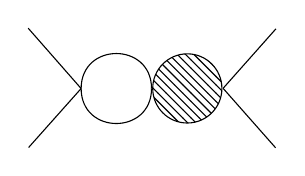
\begin{tikzpicture}[baseline=(o3.base)]
            \begin{feynman}
                \diagram[small,horizontal=o3 to o4]{
                    p1 -- o3 --[draw=none] o4 --[draw=none] o6 -- p3;
                    p2 -- o3 --[draw=none] o4 --[draw=none] o6 -- p4;
                };
                \diagram*{
                    (o3) --[half left,looseness=1.7] (o4);
                    (o3) --[half right,looseness=1.7] (o4);
                };
                \node[blob, minimum size=25pt] at ($(o4)!0.5!(o6)$) (o5);
            \end{feynman}
        \end{tikzpicture}+
        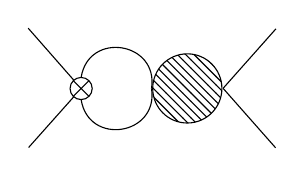
\begin{tikzpicture}[baseline=(o3.base)]
            \begin{feynman}
                \diagram[small,horizontal=o3 to o4]{
                    p1 -- o3[crossed dot, minimum size=8pt] --[draw=none] o4 --[draw=none] o6 -- p3;
                    p2 -- o3 --[draw=none] o4 --[draw=none] o6 -- p4;
                };
                \diagram*{
                    (o3) --[half left,looseness=1.7] (o4);
                    (o3) --[half right,looseness=1.7] (o4);
                };
                \node[blob, minimum size=25pt] at ($(o4)!0.5!(o6)$) (o5);
            \end{feynman}
        \end{tikzpicture}+
        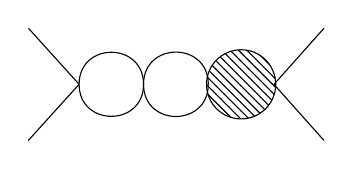
\begin{tikzpicture}[baseline=(o3.base)]
            \begin{feynman}
                \diagram[small,horizontal=o3 to o4]{
                    p1 -- o1 --[draw=none] o3 --[draw=none] o4 --[draw=none] o6 -- p3;
                    p2 -- o1 --[draw=none] o3 --[draw=none] o4 --[draw=none] o6 -- p4;
                };
                \diagram*{
                    (o1) --[half left,looseness=1.7] (o3);
                    (o1) --[half right,looseness=1.7] (o3);
                    (o3) --[half left,looseness=1.7] (o4);
                    (o3) --[half right,looseness=1.7] (o4);
                };
                \node[blob, minimum size=25pt] at ($(o4)!0.5!(o6)$) (o5);
            \end{feynman}
        \end{tikzpicture}
    \end{align*}
    with one-loop counterterm. 
    
    The integral equals to 
    \begin{align}
        \mathcal{I}&=\int\mmd[d+1]{k}\frac{i}{k^0-\frac{\vb{k}^2}{2m}+i\epsilon}\frac{i}{k^0-P^0-\frac{\abs{\vb{k-P}}^2}{2m}+i\epsilon}\\
        &=\int\mmd[d]{\vb{k}}\frac{i}{P^0-\frac{\vb{k}^2}{2m}-\frac{\abs{\vb{k-P}}^2}{2m}+2i\epsilon}\\
        &=\int\mmd[d]{\vb{k}}\frac{mi}{p^2-\vb{k}^2+i\epsilon}\\
    \end{align}

    \bibliography{../Bib}
    \bibliographystyle{apsrev4-1}
\end{document}